\documentclass[dvipdfmx,20pt,notheorems,t]{beamer}
\usepackage{minijs}
\renewcommand{\kanjifamilydefault}{\gtdefault}
\usetheme{boxes}
\usefonttheme{professionalfonts}
\setbeamertemplate{frametitle}[default][left]
\setbeamercovered{transparent}
\setbeamertemplate{footline}[page number]
\setbeamerfont{footline}{size=\normalsize,series=\bfseries}
\setbeamercolor{footline}{fg=black,bg=black}

\title[(nil)]{(nil)}
\author[@n\_IMRC]{\textbf{@n\_IMRC}}
\institute[Namiki Secondary School]{並木中等教育学校}
\date{\today}
\begin{document}
\begin{frame}[plain]\frametitle{}
\titlepage
\end{frame}

\begin{frame}\frametitle{自己紹介}
\begin{itemize}
\item 杉崎 行優
\item 並木中等教育学校 5年次
\item Makefileガチ勢
\item Twitter: @n\_IMRC
\item Yo: IMRC
\item Github: Terminus-IMRC
\item その他: http://imrc.noip.me/
\end{itemize}
\end{frame}

\begin{frame}\frametitle{今日話す内容}
\begin{itemize}
\item 45分余裕でしょ〜〜〜
\item (話す内容は考えていない)
\item 死
\end{itemize}
\end{frame}
\begin{frame}\frametitle{今日話す内容}
\begin{itemize}
\item 筑波大学のスーパーコンピュータを利用して色々した話
\begin{itemize}
\item とりあえず30分くらいは持つかも
\item 筑波大学で話すのに丁度いい内容
\item (そんなに実験してないし細かいところ触ってないけど大丈夫かな)
\item ...
\end{itemize}
\end{itemize}
\end{frame}
\begin{frame}\frametitle{今日話す内容}
\begin{figure}[htb]
\centering
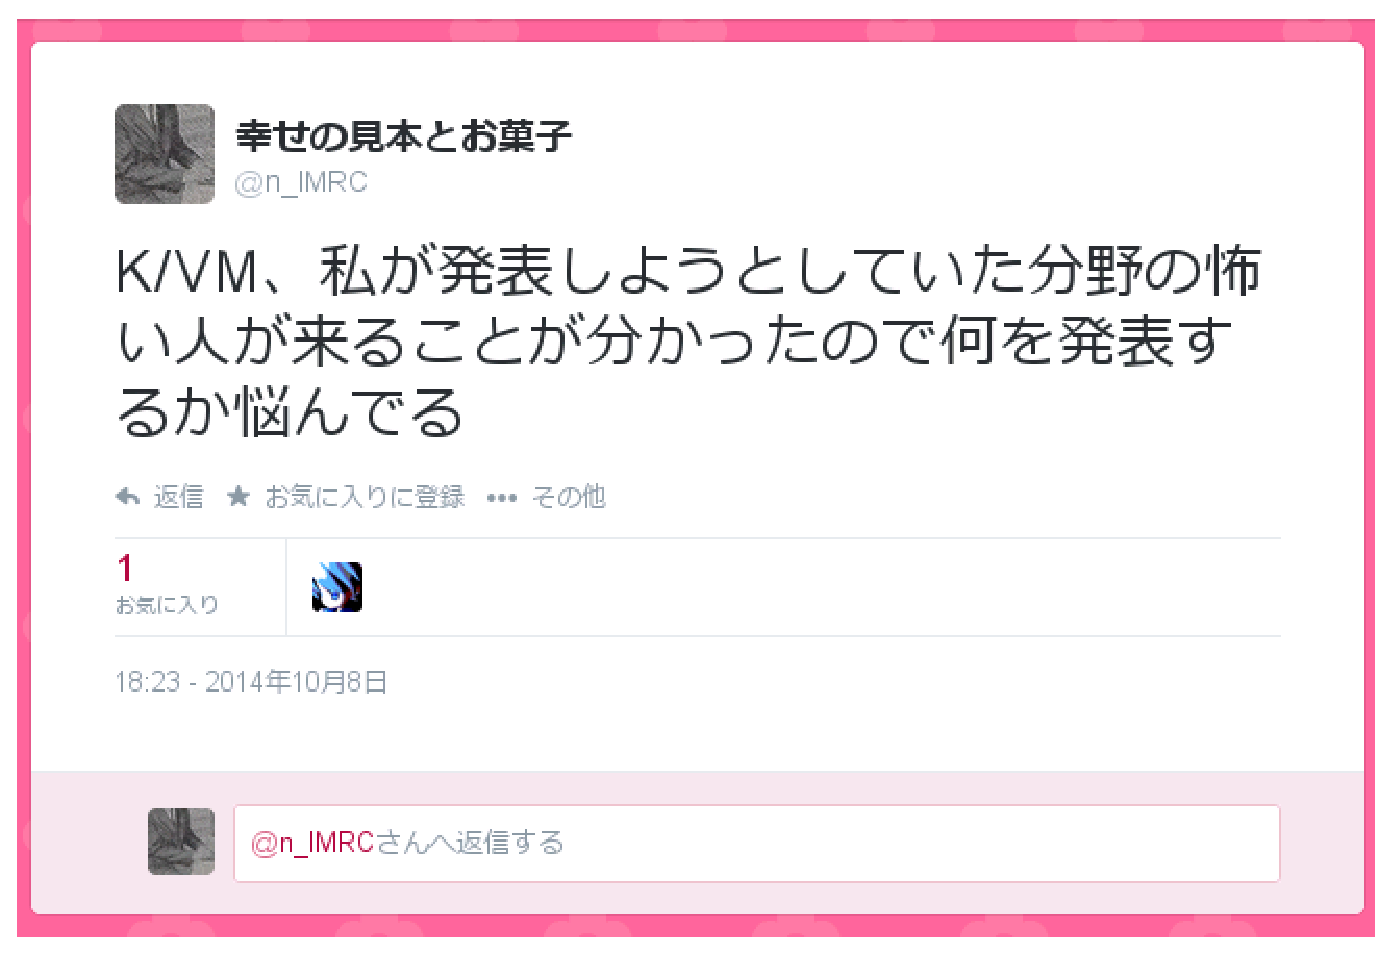
\includegraphics[width=\textwidth]{1.eps}
\end{figure}
\end{frame}
\begin{frame}\frametitle{今日話す内容}
違うテーマにしよう。うん。
\end{frame}
\begin{frame}\frametitle{今日話す内容}
\begin{itemize}
\item USBキーボード to Bluetooth コンバータの製作...?
\begin{itemize}
\item 45分持たない
\item ボツ
\end{itemize}
\end{itemize}
\end{frame}
\begin{frame}\frametitle{今日話す内容}
\begin{figure}[htb]
\centering
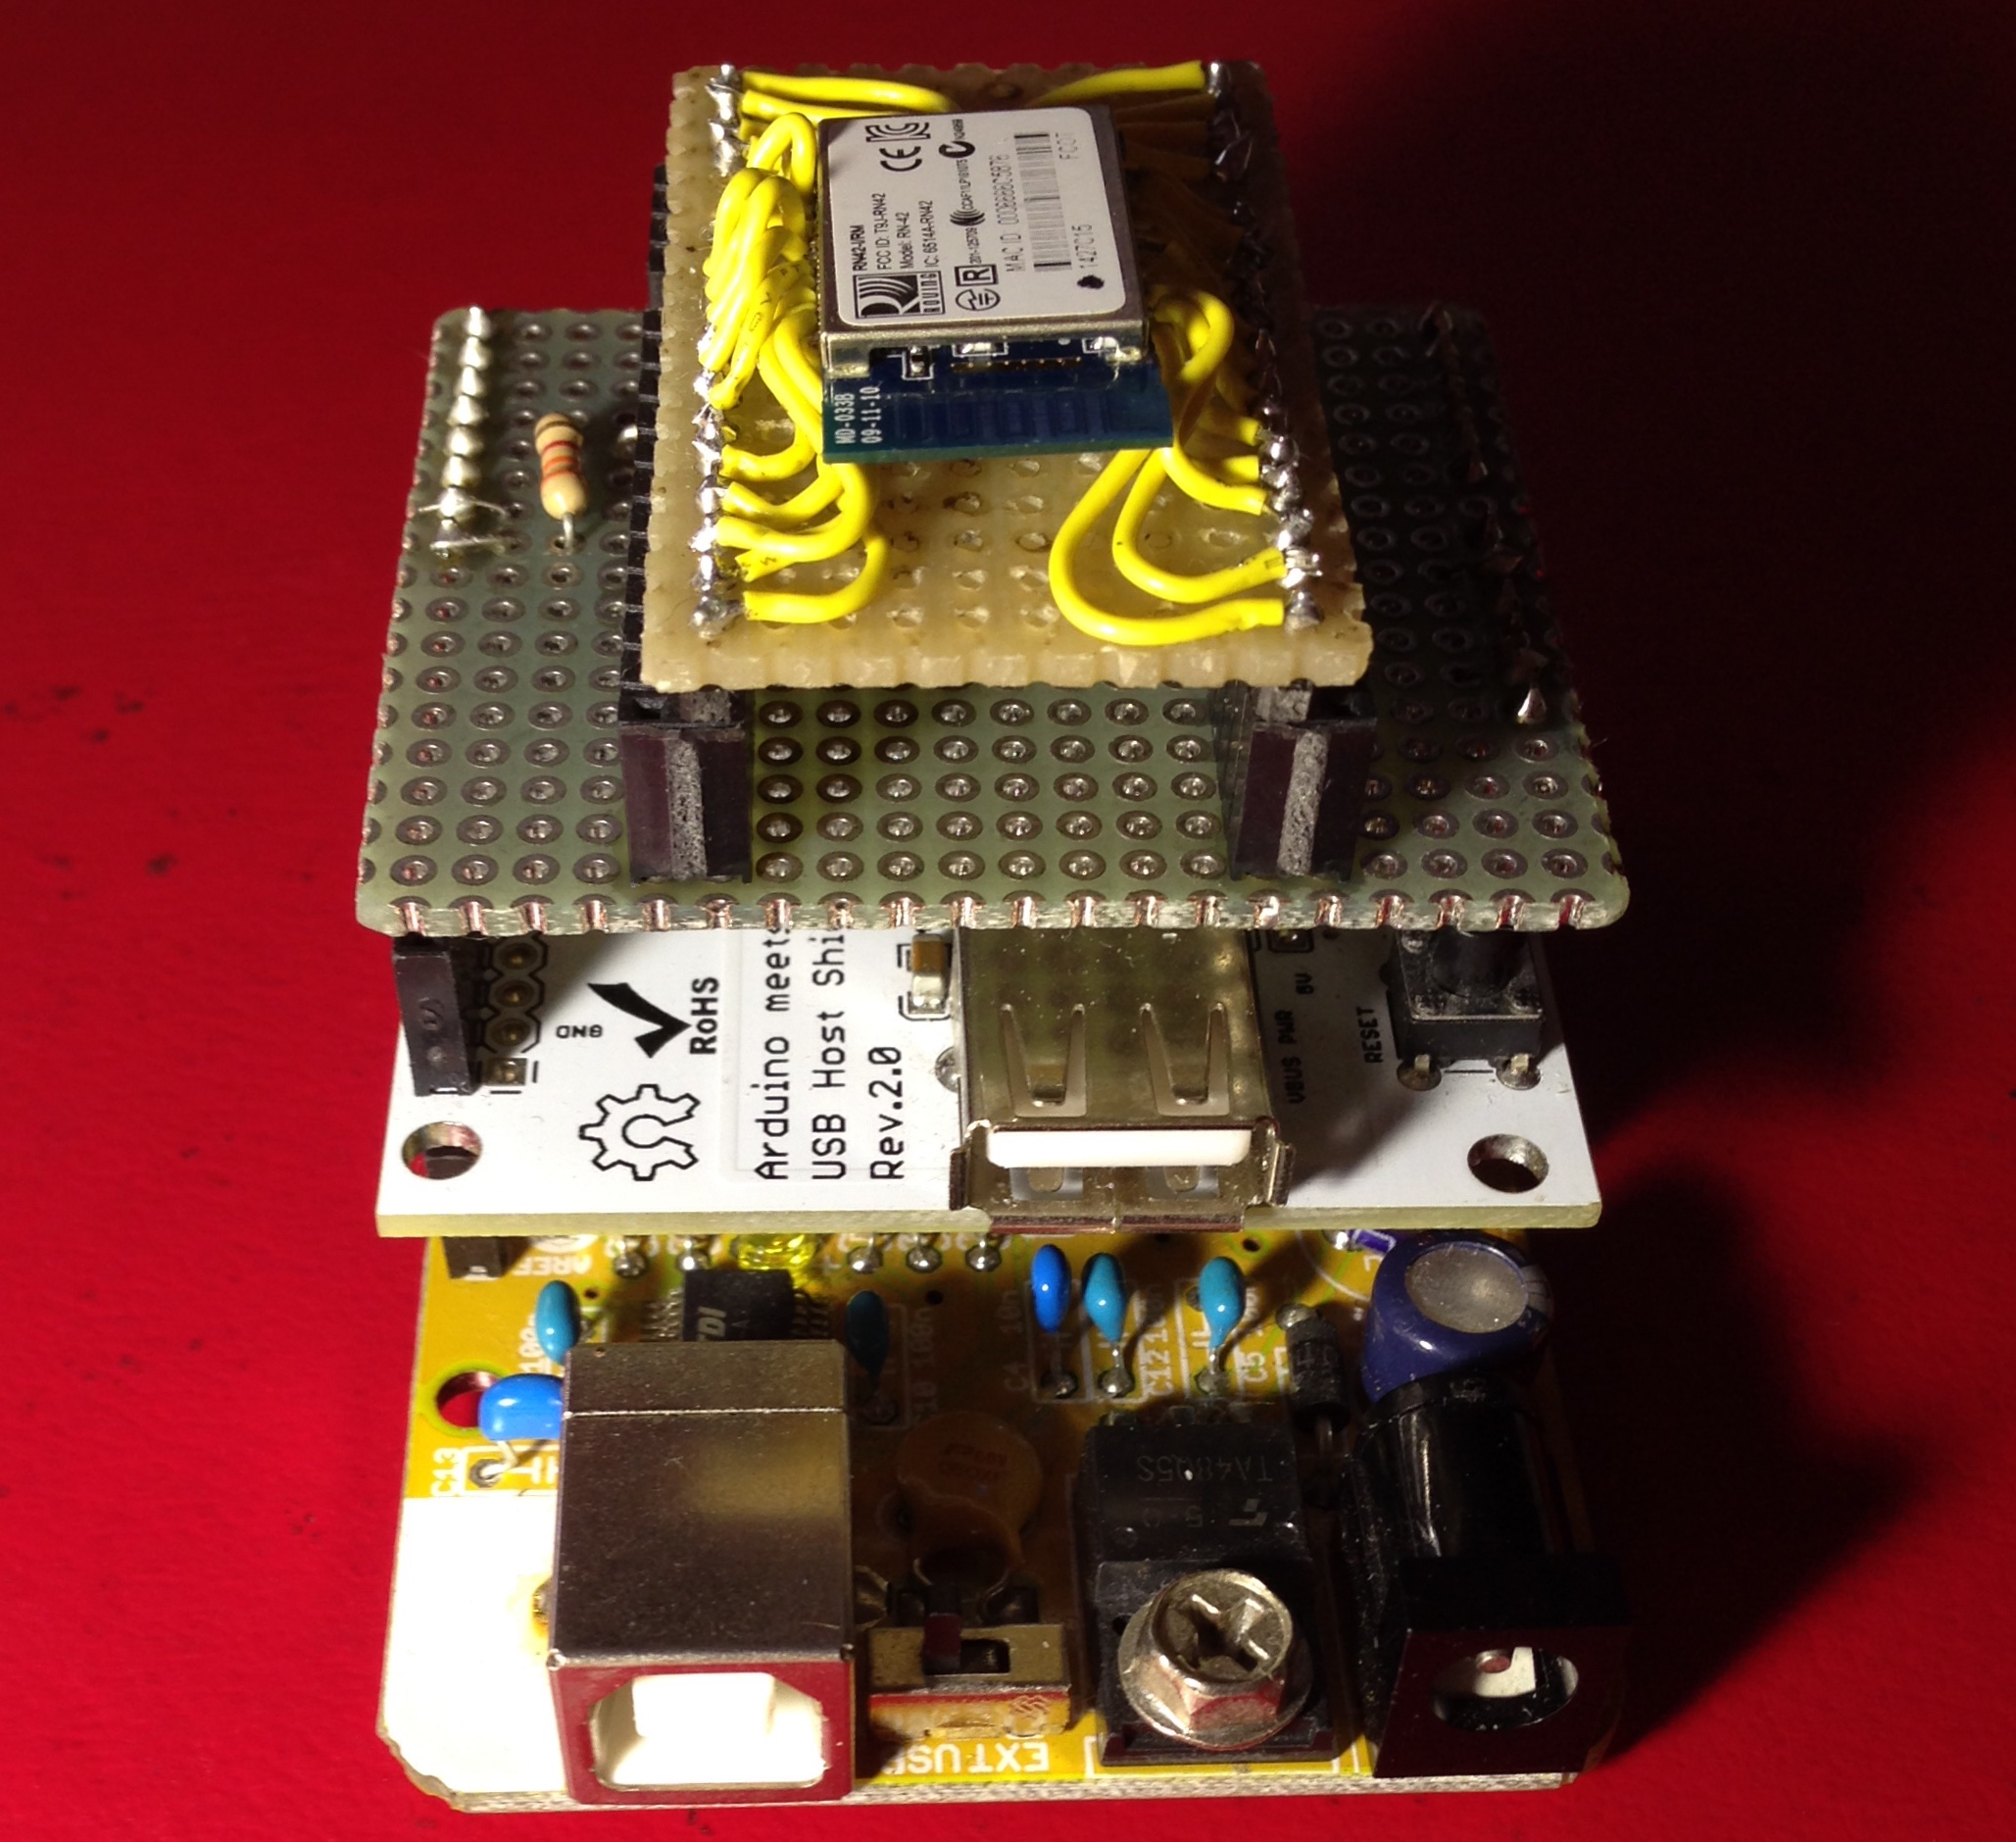
\includegraphics[width=0.7\textwidth]{bt.eps}
\end{figure}
\end{frame}

\begin{frame}\frametitle{今日話す内容}
\begin{itemize}
	\item initスクリプトを書いてRaspberryPiのOSをUSB HDDから起動できるようにした話...?
	\begin{itemize}
		\item 新規性がない
		\item 45分持たない
		\item ボツ
	\end{itemize}
\end{itemize}
\end{frame}
\begin{frame}\frametitle{今日話す内容}
\begin{itemize}
	\item framebufferをpngやjpegに変換するプログラムを書き、mjpg\_streamer経由でストリーミングできるようにした話...?
	\begin{itemize}
		\item 最近のTLの風潮はsixel
		\item 45分持たない
		\item ボツ
	\end{itemize}
\end{itemize}
\end{frame}

\begin{frame}\frametitle{今日話す内容}
\begin{itemize}
\item 45分の内に複数テーマを話す...?
\begin{itemize}
\item 45分話したかった方に申し訳ない
\begin{itemize}
\item マサカリは怖いけど...
\end{itemize}
\end{itemize}
\end{itemize}
\end{frame}
\begin{frame}\frametitle{今日話す内容}
\begin{figure}[htb]
\centering
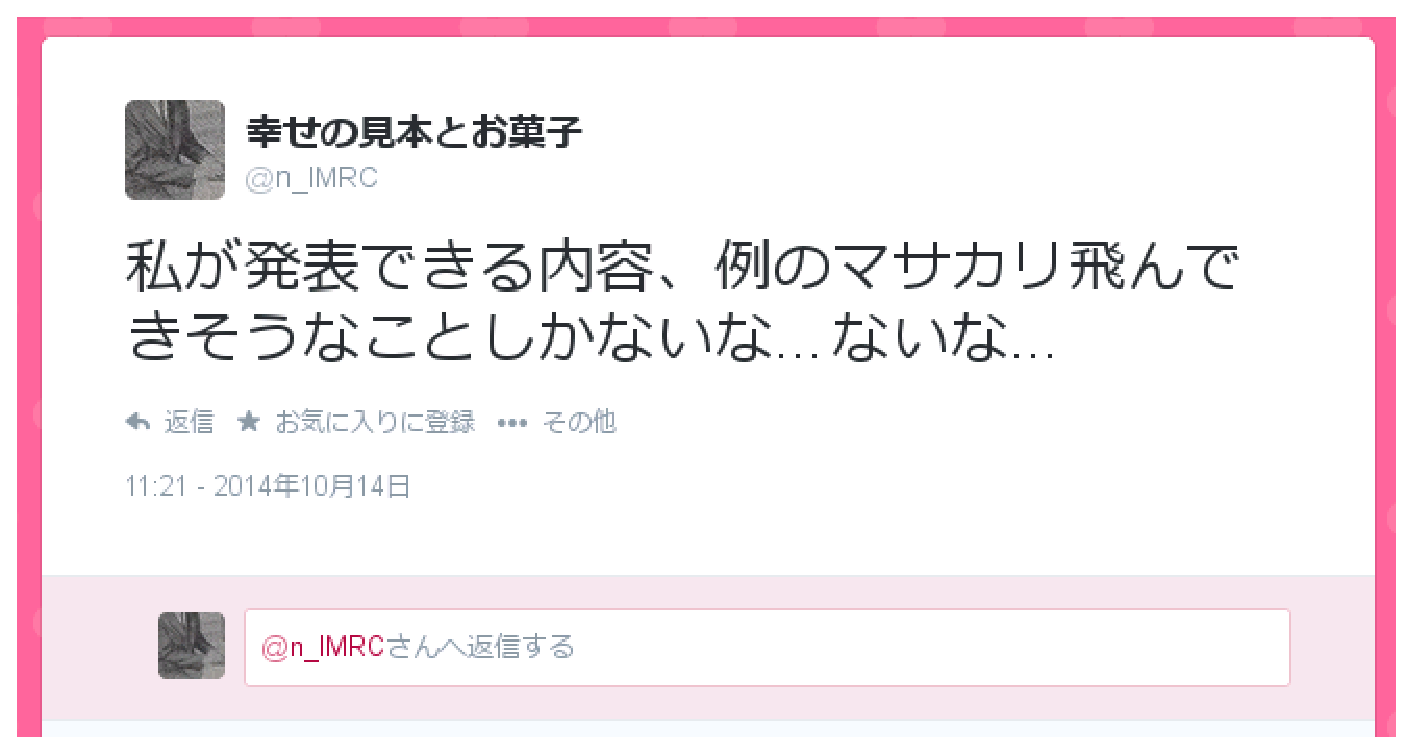
\includegraphics[width=\textwidth]{2.eps}
\end{figure}
\end{frame}
\begin{frame}\frametitle{今日話す内容}
\centering
\vspace*{\fill}
私が筑波大学の \\
スーパーコンピュータを使用して \\
出した成果 \\
(「$n$次魔方陣のプログラムを書き、並列化した話」と「XeonPhiを触って感じたこと」)
\vspace*{\fill}
\end{frame}

\begin{frame}\frametitle{並列計算}
\begin{itemize}
\item 複数のCPUやスレッドで分散して処理
\item 実行時間の短縮が目的
\begin{itemize}
\item 理想は \textbf{(元の実行時間)/n}
\item 通信やアルゴリズムのオーバーヘッドにより、現実的に不可能
\end{itemize}
\end{itemize}
\end{frame}

\begin{frame}\frametitle{並列計算の概念図}
\begin{figure}[htb]
\centering
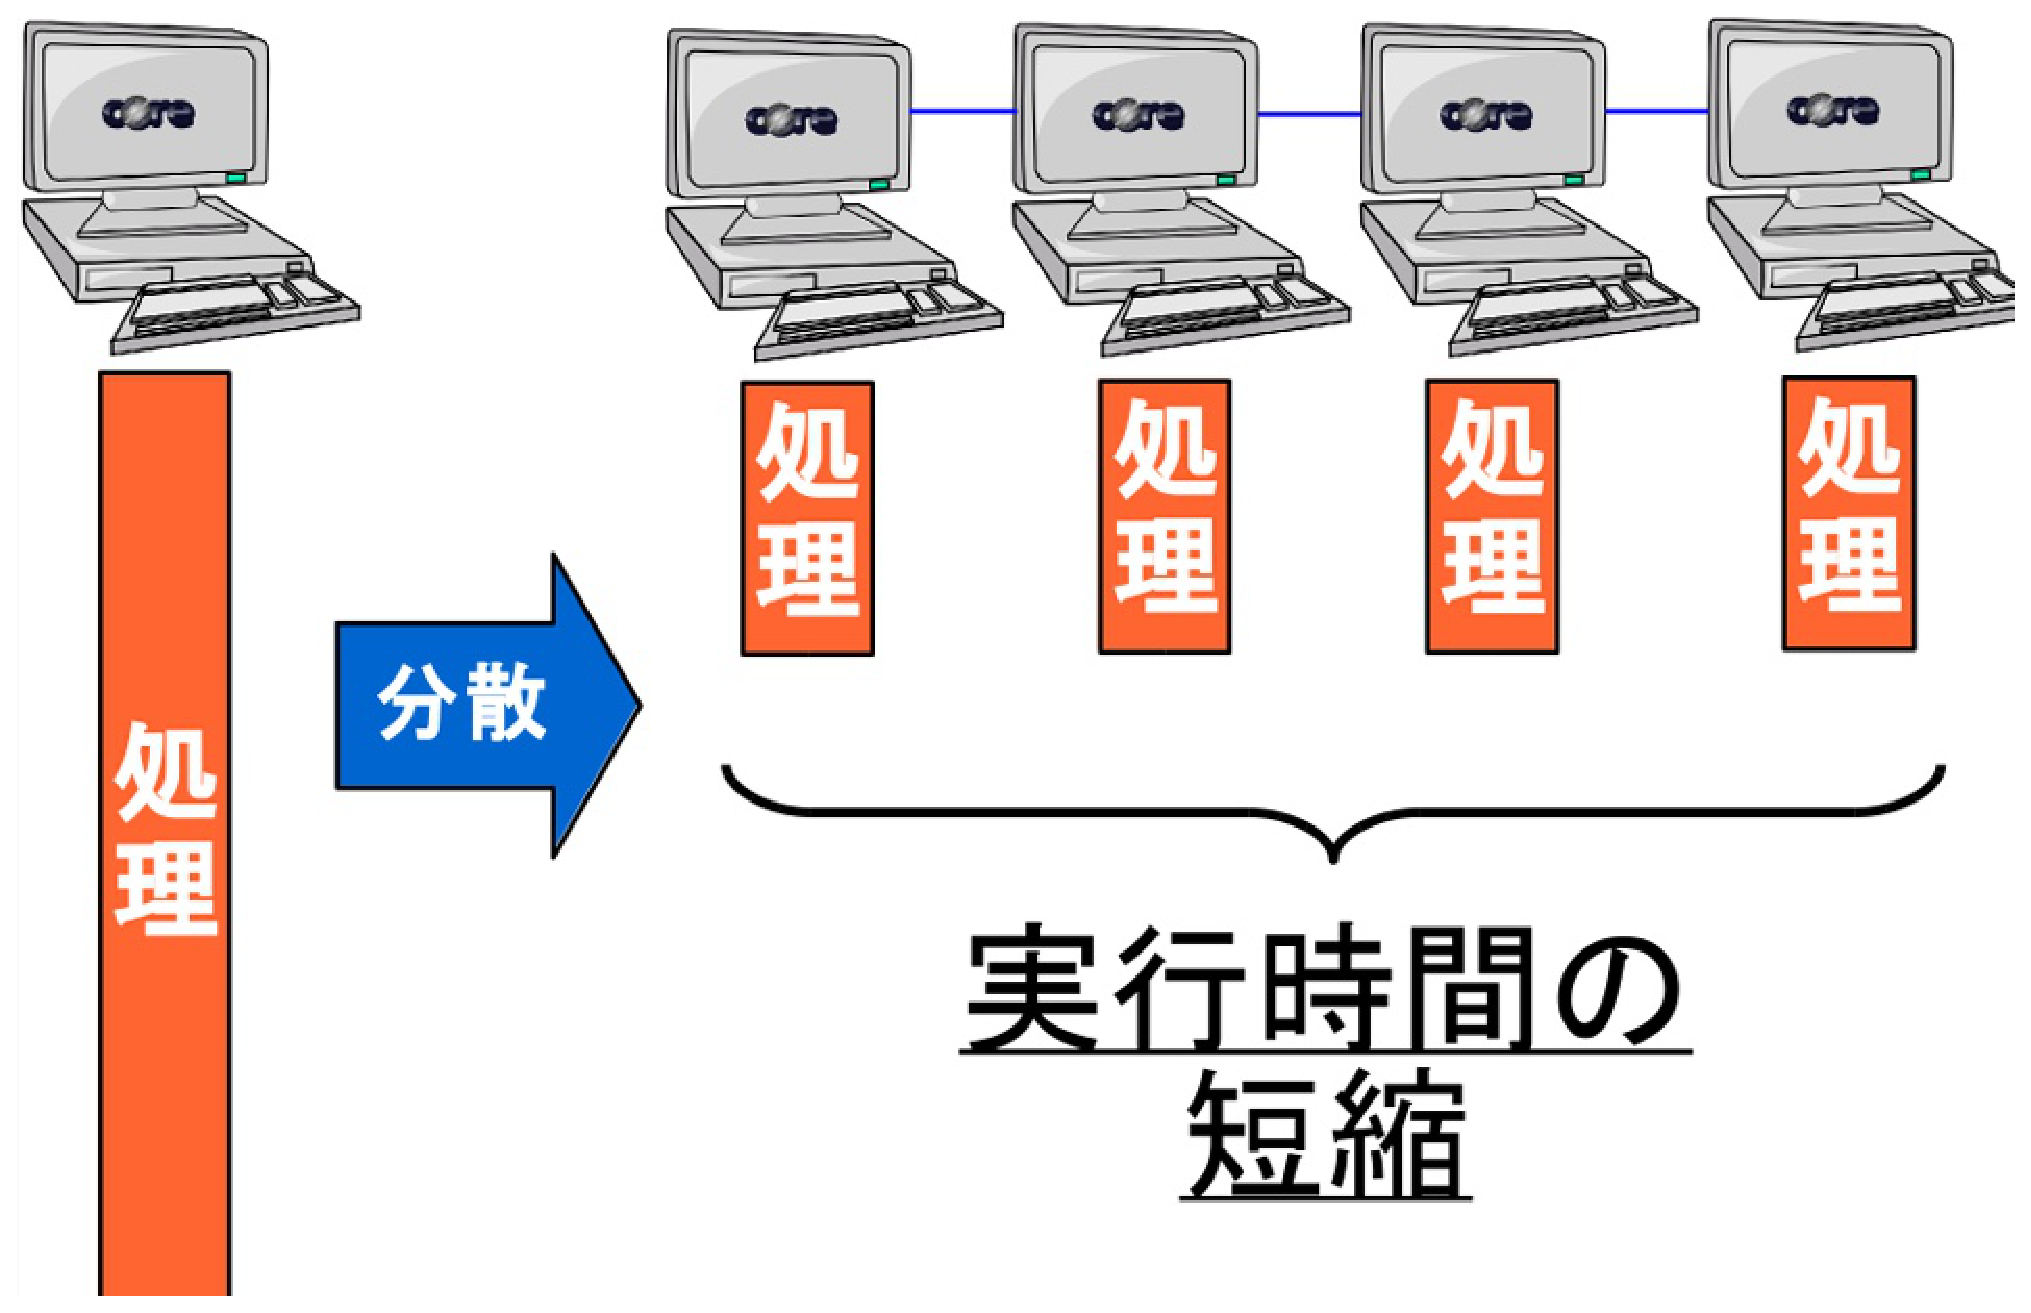
\includegraphics[width=\textwidth]{master-worker.eps}
\end{figure}
\end{frame}

\begin{frame}\frametitle{並列計算のための環境}
\begin{itemize}
\item 数値計算においてはMPI, OpenMP, pthread等の高レベルなライブラリ
\item 筑波大学がdirectiveベースの、MPIによる並列言語XcalableMPを開発中
\item CPU間通信にNUMAを使うことも
\end{itemize}
\end{frame}

\begin{frame}\frametitle{スーパーコンピュータ}
\begin{itemize}
\item (多少高性能な)コンピュータの集まり
\begin{itemize}
\item 並列計算もしくは並行計算
\end{itemize}
\item 現在、筑波大学はHA-PACSとCOMAを運用している
\begin{itemize}
\item 昨年度までT2K-Tsukubaが運用されていた
\end{itemize}
\end{itemize}
\end{frame}

\begin{frame}\frametitle{T2K-Tsukuba}
\small
1ノード: quad-core AMD Opteron $\times$ 4
\begin{figure}[htb]
\centering
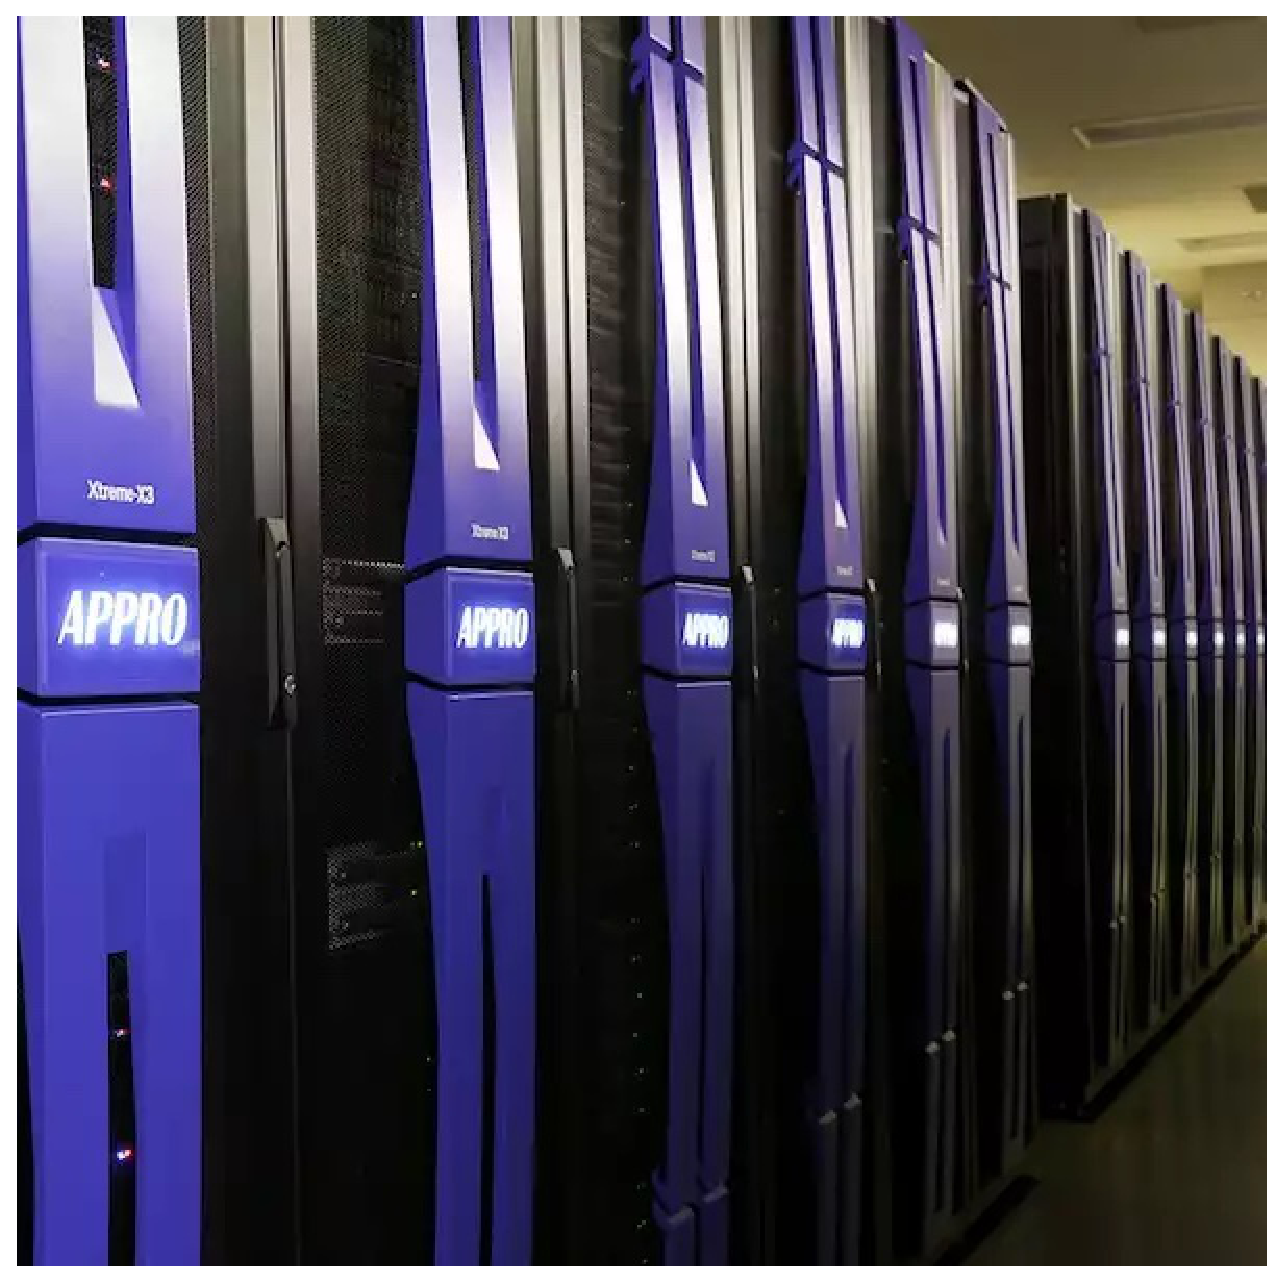
\includegraphics[height=0.6\textheight]{t2kt.eps}
\end{figure}
\end{frame}

\begin{frame}\frametitle{HA-PACS}
\small
1ノード: NVIDIA M2090(Fermi) $\times$ 4
\begin{figure}[htb]
\centering
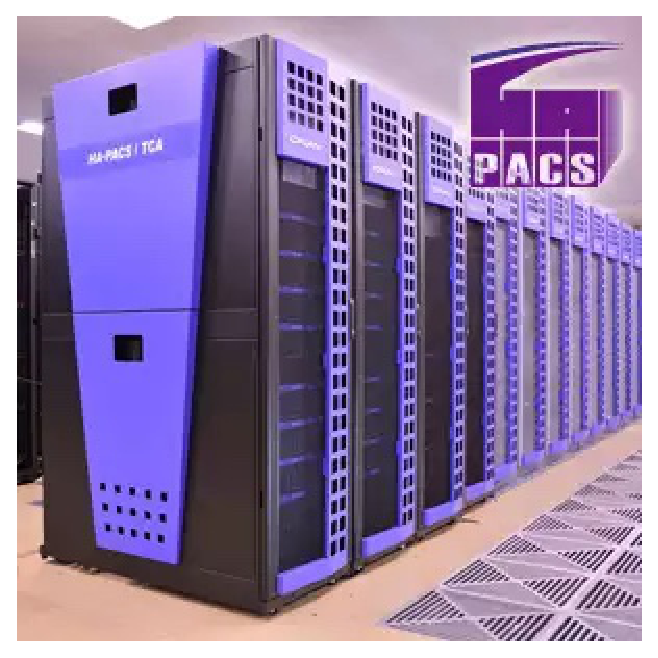
\includegraphics[height=0.6\textheight]{hapacs.eps}
\end{figure}
\end{frame}

\begin{frame}\frametitle{COMA}
\small
1ノード: Intel Xeon Phi $\times$ 2
\begin{figure}[htb]
\centering
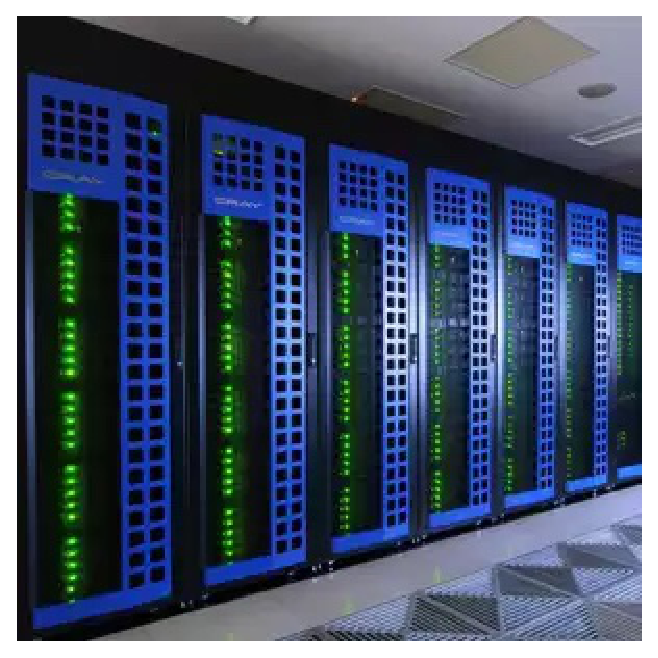
\includegraphics[height=0.6\textheight]{coma.eps}
\end{figure}
\end{frame}

\begin{frame}\frametitle{学際共同利用とは}
\begin{itemize}
\item 筑波大学学際共同利用
\item 申請に通れば1年間無料でスパコンを利用できる
\begin{itemize}
\item (最低でも)5TBのディスクスペース
\item 申請資格: {\tiny 研究員, 大学または高専の学生, 研究機関に所属する者,} \textbf{その他センター長が認めた者}
\end{itemize}
\end{itemize}
\end{frame}

\begin{frame}\frametitle{学際共同利用での私の成果}
\begin{itemize}
\item 平成24年度: $n$次魔方陣全解数え上げプログラムの並列化と性能解析
\item 平成25年度: $n$次魔方陣全解数え上げプログラムのメニーコア化
\end{itemize}
\end{frame}

\begin{frame}\frametitle{学際共同利用での私の成果}
\centering
\large
$n$次魔方陣全解 \\
数え上げプログラムの \\
並列化と性能解析
\end{frame}

\begin{frame}\frametitle{目的}
一般的な整数問題である「$n$次魔方陣」の全解探索を超並列処理によって行う試み
\end{frame}

\begin{frame}\frametitle{$n$次魔方陣}
\begin{itemize}
\item 縦$n$、横$n$、計$n^2$マス
\item $1$から$n^2$がユニークに入る
\item 縦・横・斜めの列それぞれの合計がすべて等しい
\end{itemize}
\centering
\begin{displaymath}
L=\frac{1}{n}\sum_{i=1}^{n^2}i
\end{displaymath}
\end{frame}

\begin{frame}\frametitle{$n$次魔方陣}
\begin{figure}[htb]
\centering
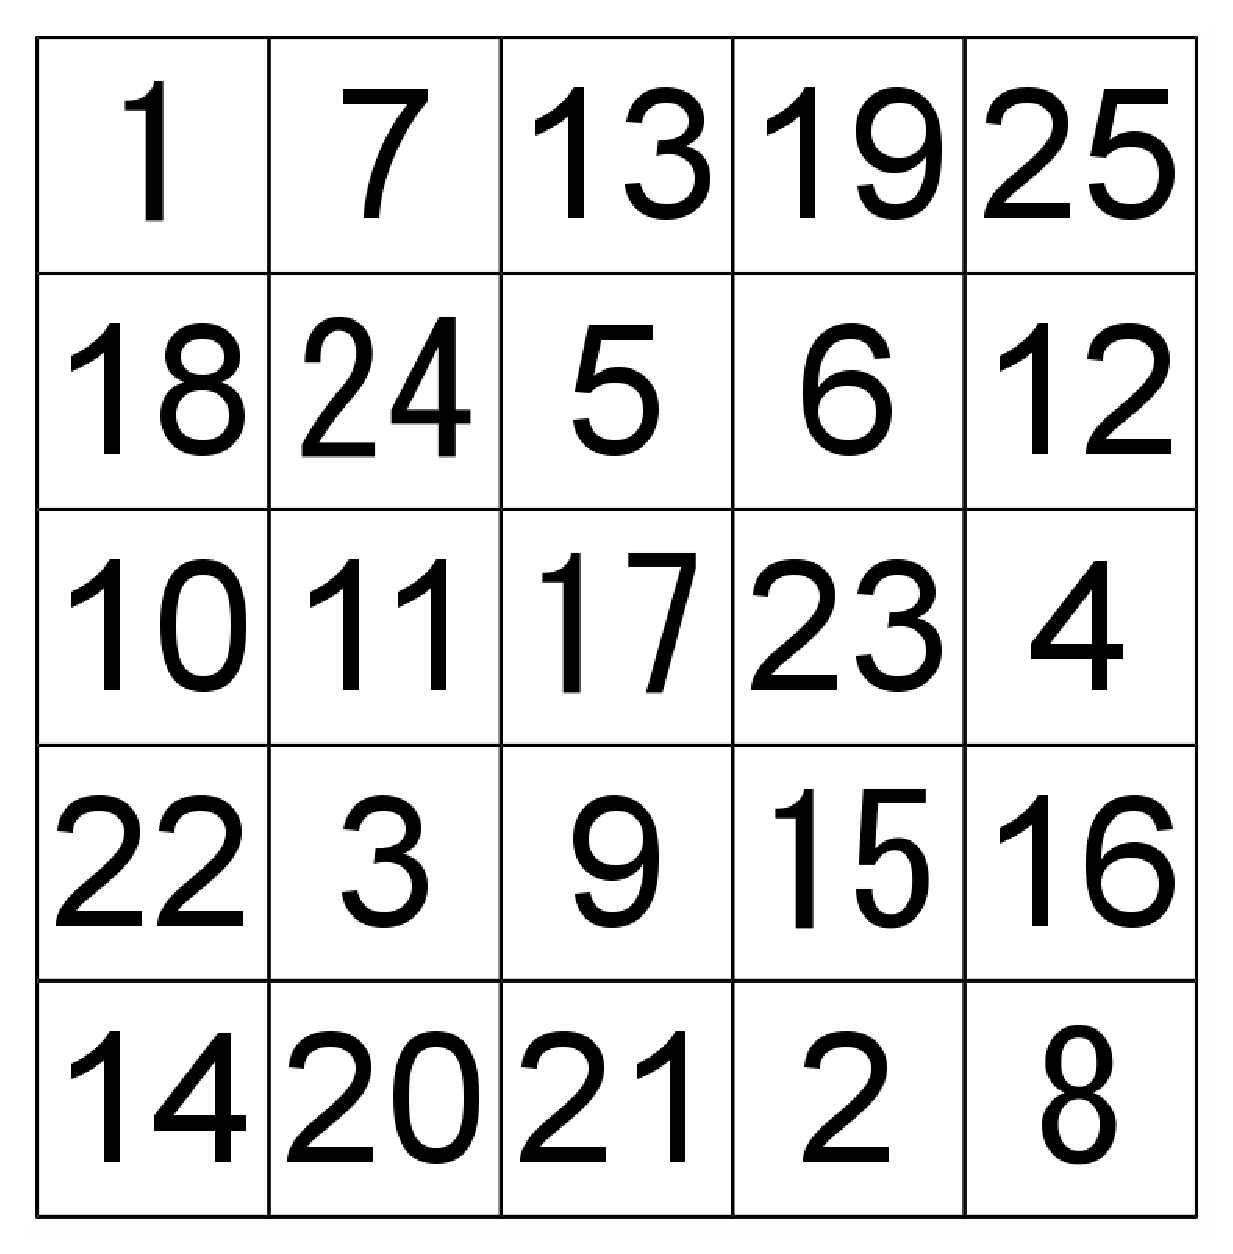
\includegraphics[height=0.7\textheight]{ms.eps}
\end{figure}
\end{frame}

\begin{frame}\frametitle{目的}
\begin{itemize}
\item $n$の増大に伴い、階乗的に増加する探索空間を数学的に絞り込む
\item 動的負荷分散処理をMPIによりプログラムし効率的処理を行う
\end{itemize}
\end{frame}

\begin{frame}\frametitle{目的}
\begin{itemize}
\item 当初目的は、未だに解が求まっていない$n=6$の求解であったが、計算リソース上困難
\begin{itemize}
\item 目標を$n=5$(解が求まっている)に対して正しく動作するプログラムと、その動的負荷分散機能の検証及び評価に修正
\end{itemize}
\end{itemize}
\end{frame}

\begin{frame}\frametitle{計算環境}
\begin{itemize}
\item 筑波大学学際共同利用プログラムにより、筑波大学のスーパーコンピュータであるT2K-Tsukubaを利用
\item 32ノード上で512スレッドを実行
\item 最大連続実行時間は24時間
\end{itemize}
\end{frame}

\begin{frame}\frametitle{アルゴリズムの改良}
\begin{itemize}
\item 鏡像性、途中解から一意に求まる解、等の性質から、できるだけ計算量を絞る
\item 部分的に解けているパターンからその先の全解探索を行うよう、探索空間を木構造化
\end{itemize}
\end{frame}

\begin{frame}\frametitle{アルゴリズムの改良}
\begin{figure}[htb]
\centering
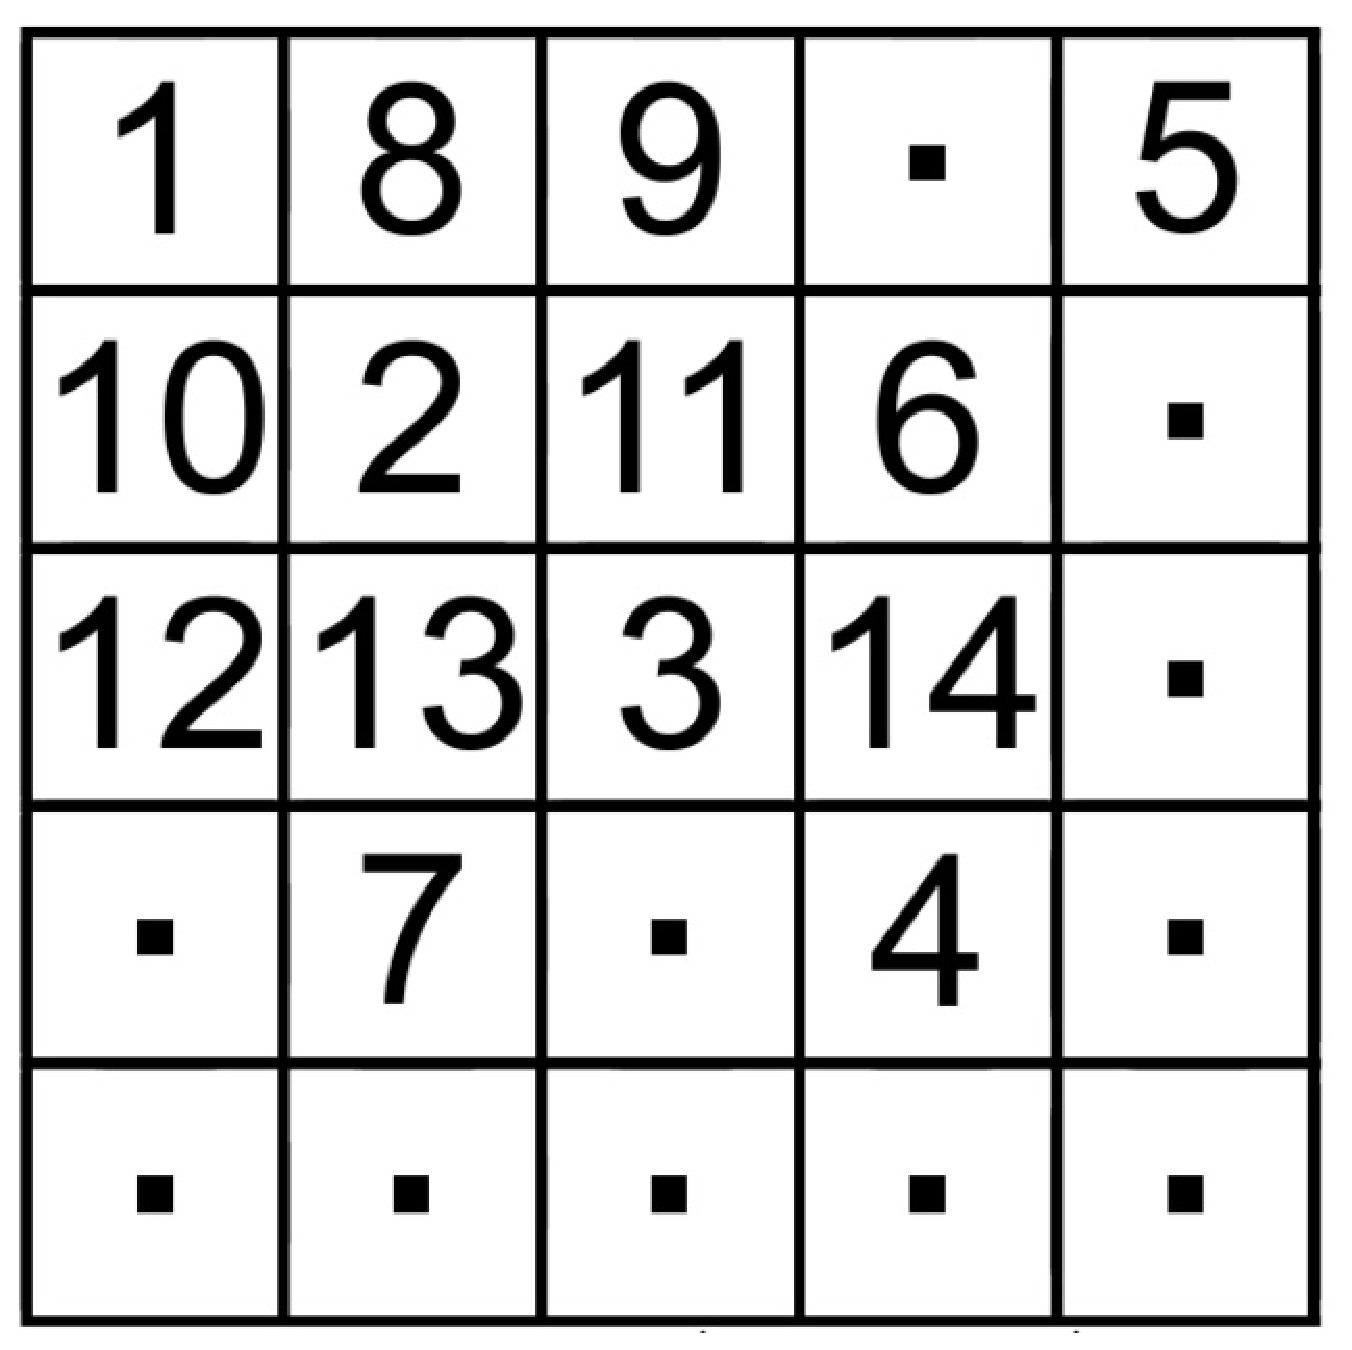
\includegraphics[height=0.7\textheight]{order.eps}
\end{figure}
\end{frame}

\begin{frame}\frametitle{アルゴリズムの改良}
\begin{itemize}
\item 部分解からの探索の計算量は事前に求められないため、動的タスクスケジューリングが必要
\item 部分解パターンの表現データが小さいのに対し、探索空間は大きいため、master-worker型並列処理が有効
\end{itemize}
\end{frame}

\begin{frame}\frametitle{master-worker型並列}
\begin{itemize}
\item masterが暇なworkerに問題を投げ、全ての候補に対する処理が終わるまで繰り返す
\end{itemize}
\end{frame}

\begin{frame}\frametitle{master-worker型並列}
\begin{figure}[htb]
\centering
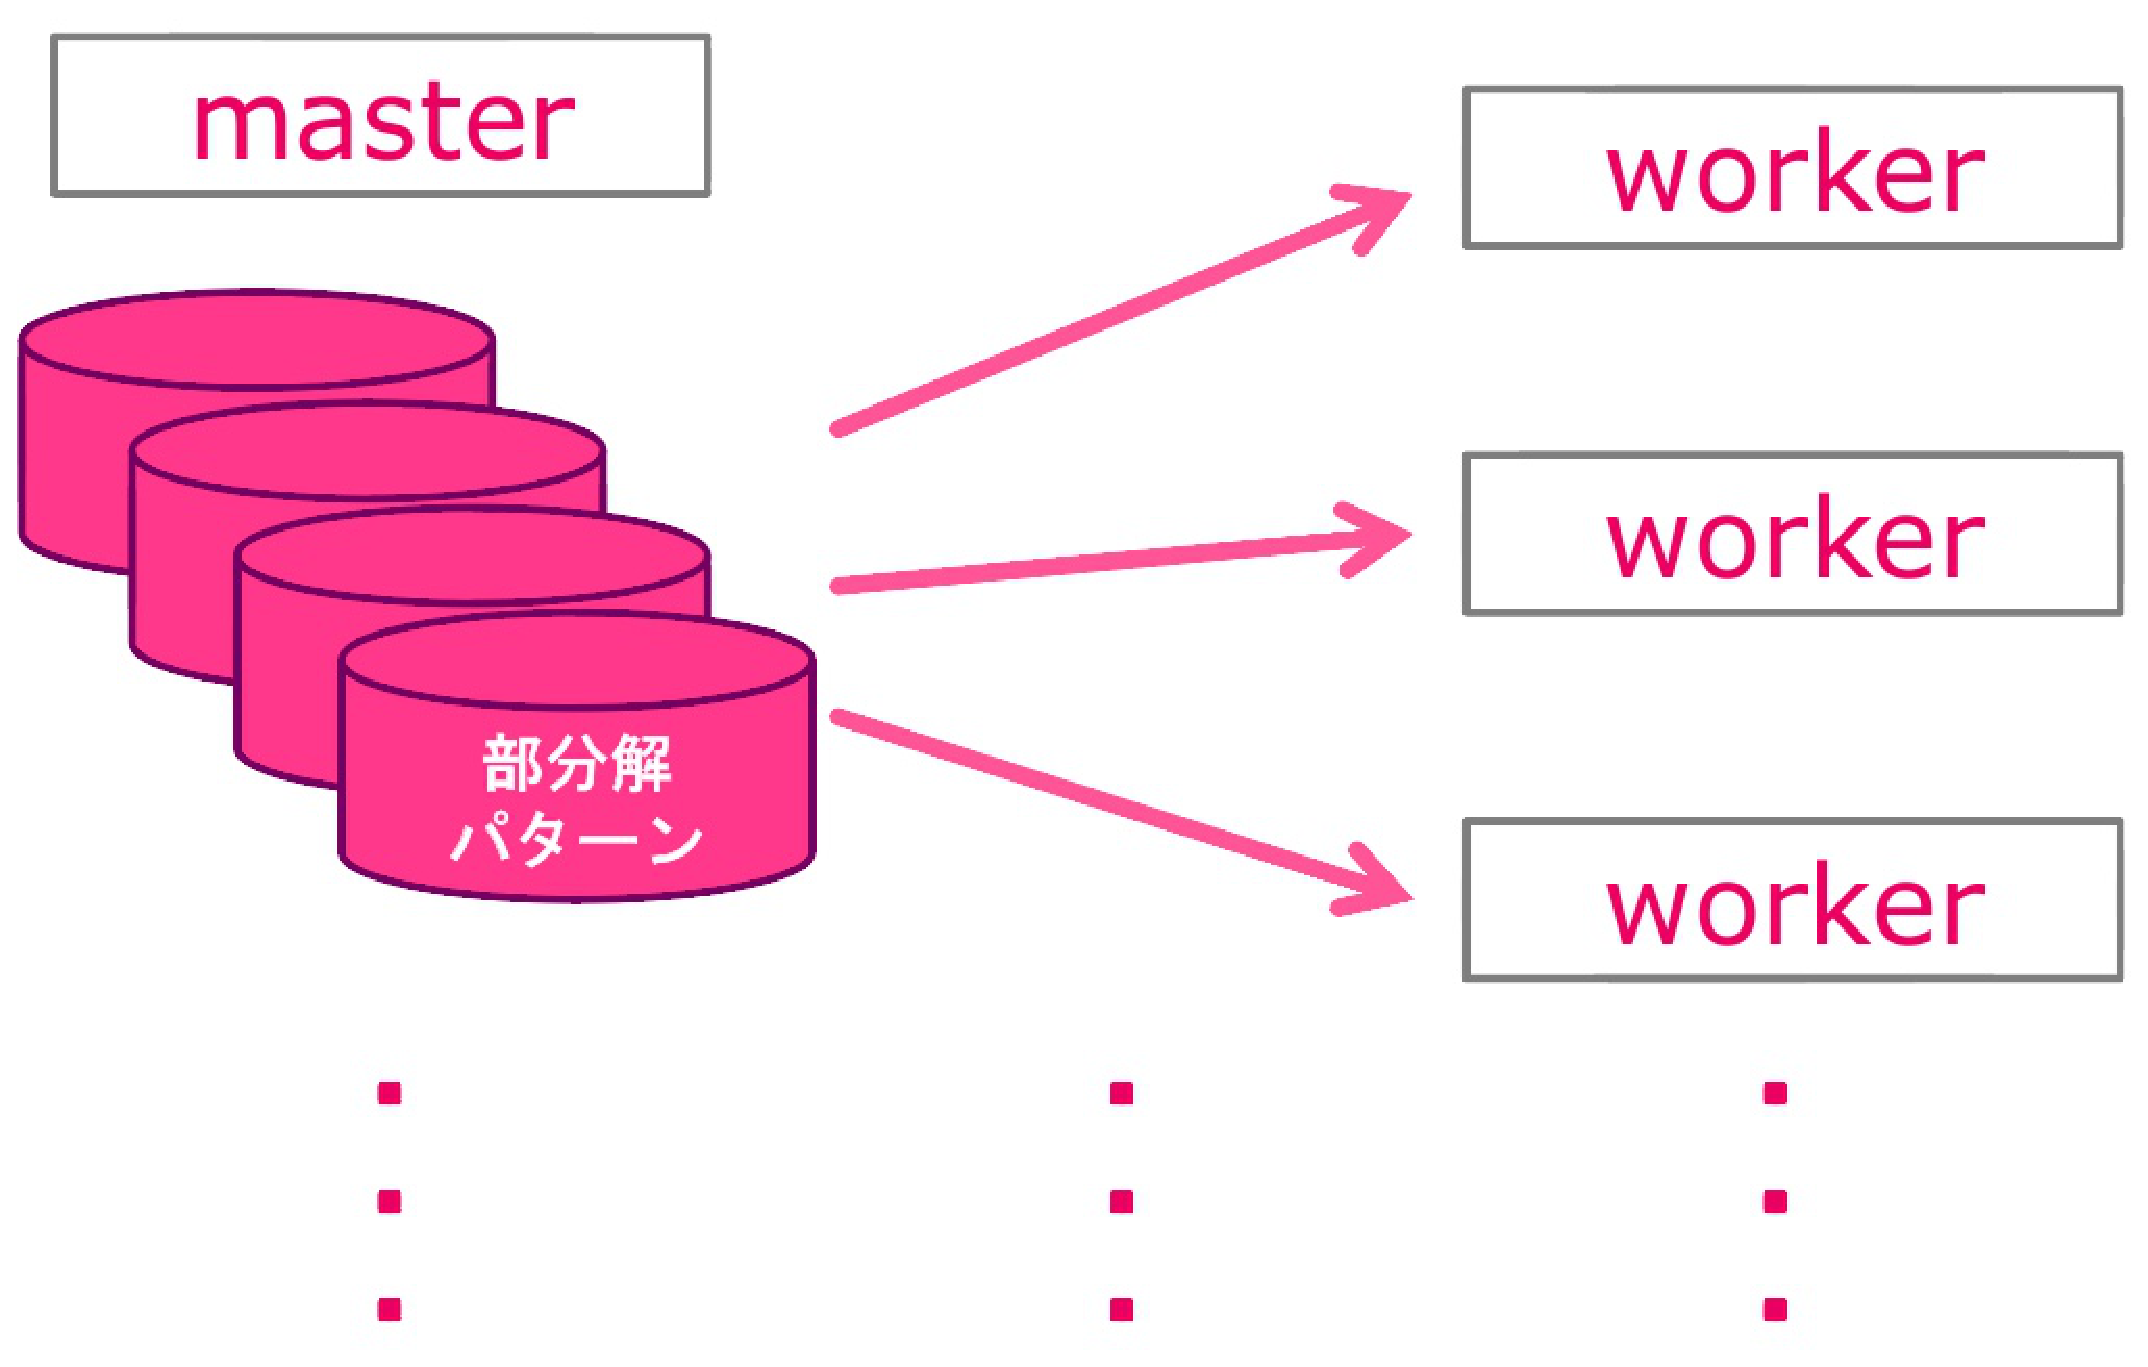
\includegraphics[height=0.7\textheight]{real-master-worker.eps}
\end{figure}
\end{frame}

\begin{frame}\frametitle{並列化時のポイント}
\begin{itemize}
\item 部分解を「25マス中$D$個まで埋まった状態」とし、このパターンをworkerに分配
\item $D$が大きいとその先の探索空間が小さく、\\ $D$が小さいとその逆
\end{itemize}
\end{frame}

\begin{frame}\frametitle{並列化時のポイント}
\begin{itemize}
\item worker数が大きいとmasterの分配処理が大きくなり、小さいとmasterはidleになりやすい
\end{itemize}
これらを踏まえ、worker数と$D$の関係の最適値を経験的に調査
\end{frame}

\begin{frame}\frametitle{今回の並列処理のイメージ}
\begin{figure}[htb]
\centering
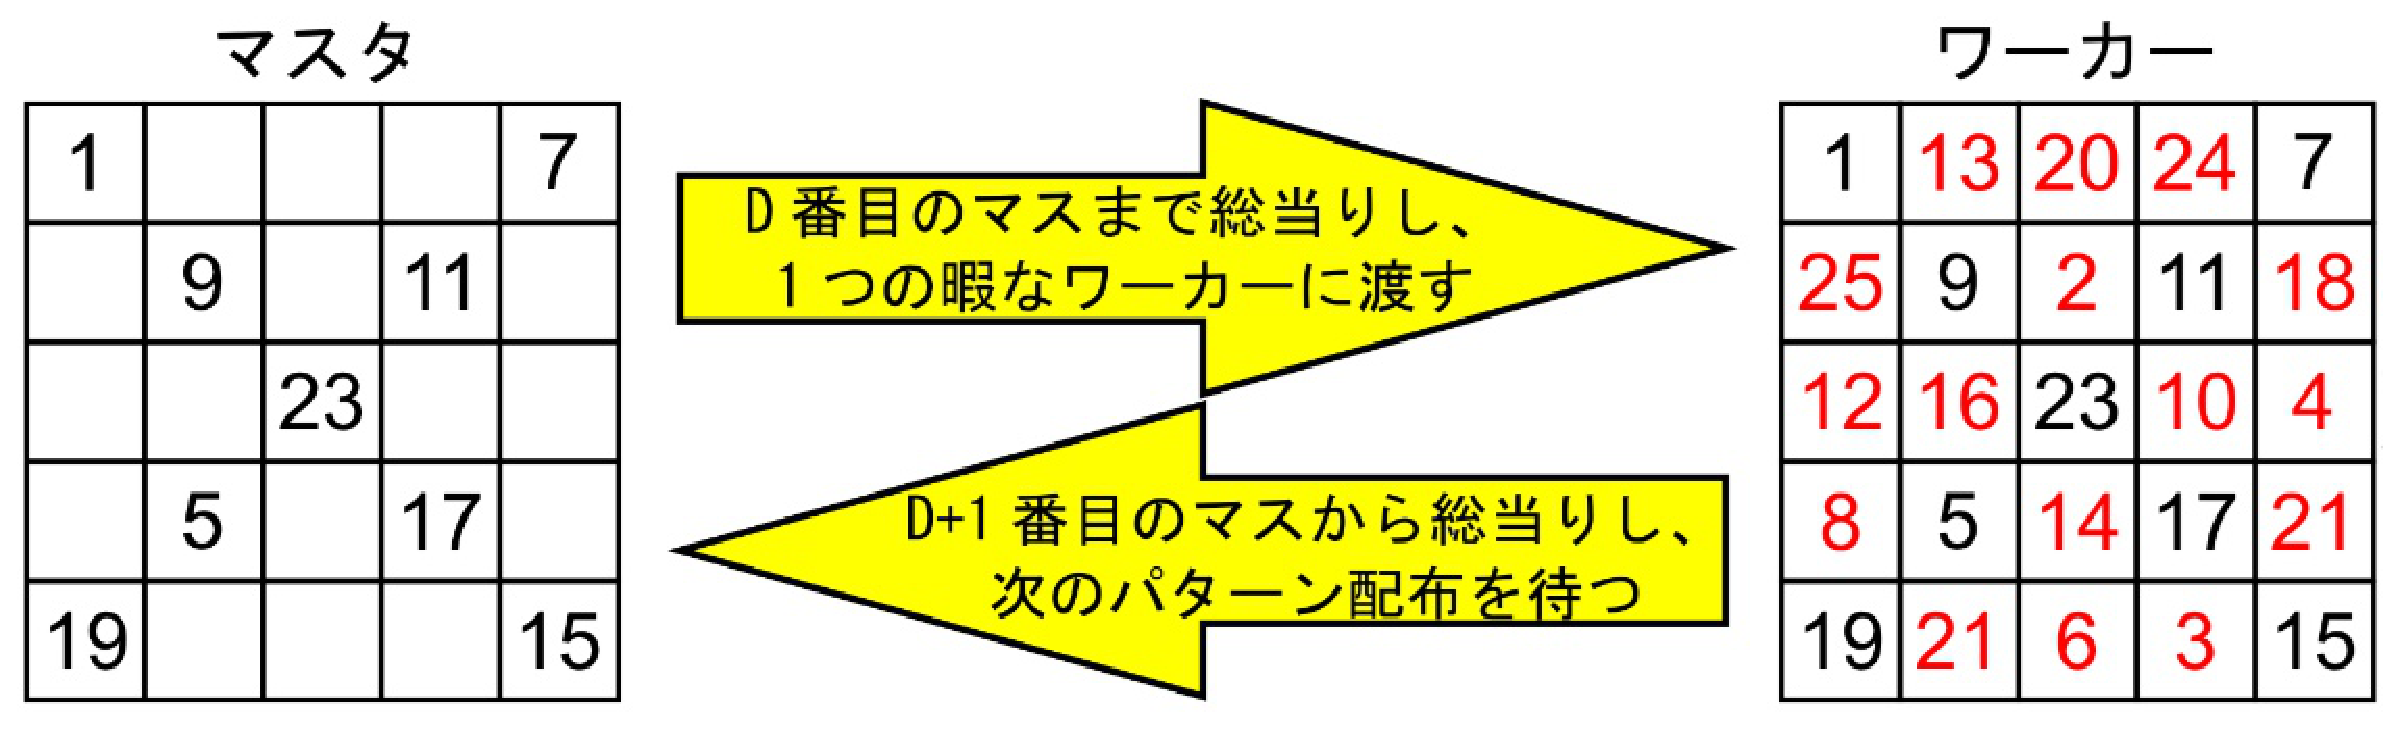
\includegraphics[width=0.9\textwidth]{master-worker-proc.eps}
\end{figure}
\end{frame}

\begin{frame}\frametitle{実験結果}
\end{frame}

\begin{frame}\frametitle{各$D$における全体処理時間}
\begin{figure}[htb]
\centering
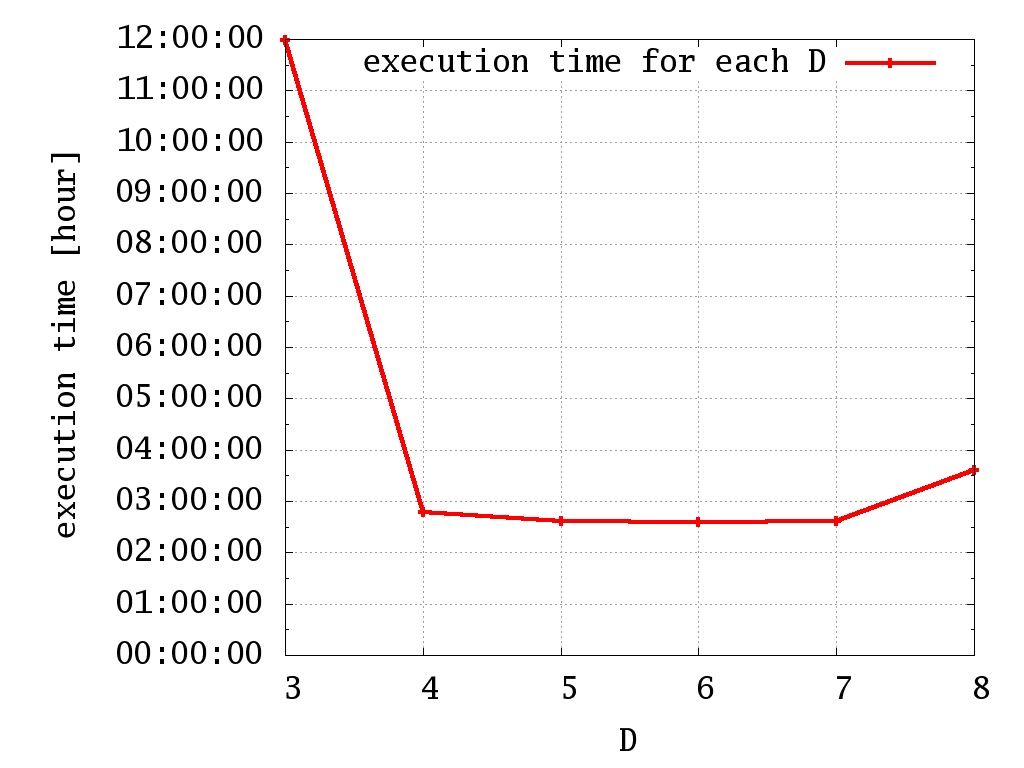
\includegraphics[width=0.8\textwidth]{alltim.eps}
\end{figure}
\end{frame}

\begin{frame}\frametitle{各workerの処理時間}
\begin{figure}[htb]
\centering
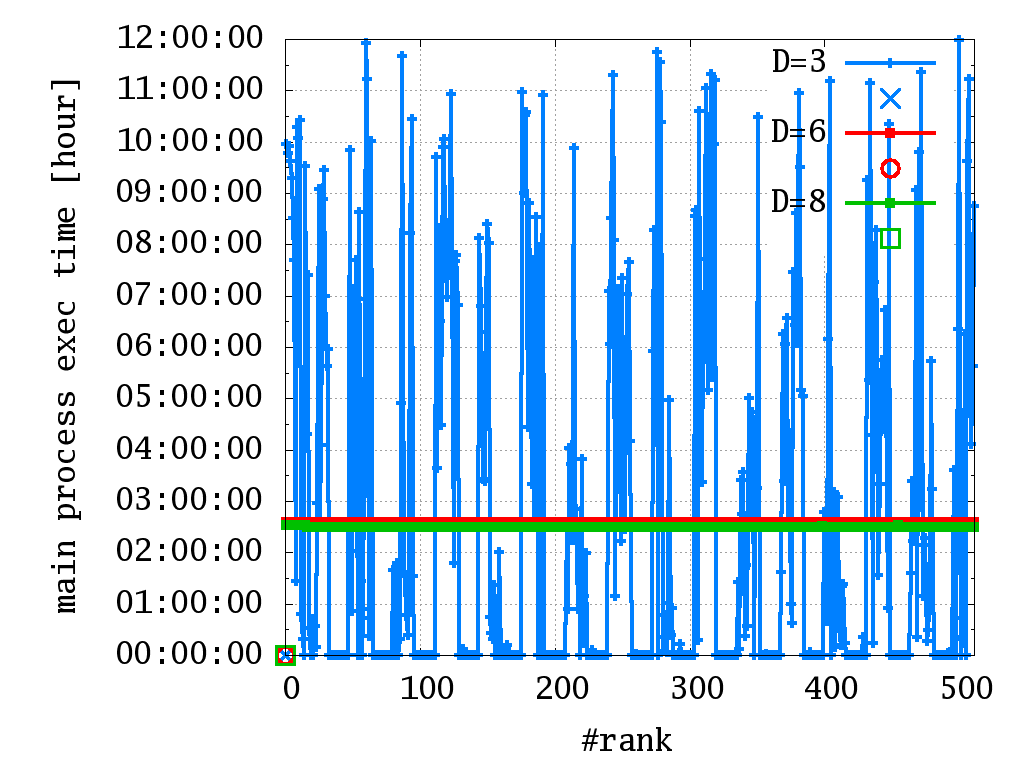
\includegraphics[width=0.8\textwidth]{sumefl.eps}
\end{figure}
\end{frame}

\begin{frame}\frametitle{各workerの通信時間}
\begin{figure}[htb]
\centering
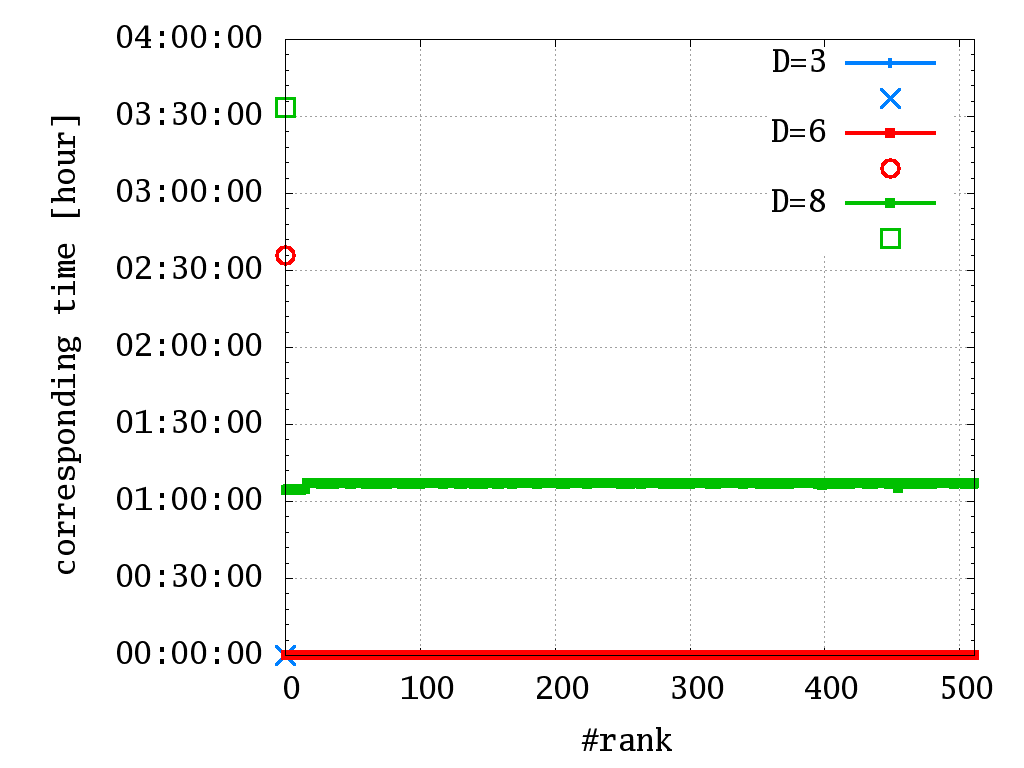
\includegraphics[width=0.8\textwidth]{sumwcr.eps}
\end{figure}
\end{frame}

\begin{frame}\frametitle{結果・考察}
\begin{itemize}
\item $D=3$では各workerの処理時間にバラつきが見られた
\item $D=8$では各workerの通信時間が比較的長い
\item $D=6$のバランスが良く、全体処理時間が最短になったのではないか
\end{itemize}
\end{frame}

\begin{frame}\frametitle{6次魔方陣への拡張}
\begin{itemize}
\item 今回のアルゴリズムをそのまま6次に拡張すると、実行に150兆年かかる見込み
\item アルゴリズムを大幅に改良しない限り現実的に不可能
\end{itemize}
\end{frame}

\begin{frame}\frametitle{学際共同利用での私の成果}
\centering
\large
$n$次魔方陣全解 \\
数え上げプログラムの \\
メニーコア化
\end{frame}

\begin{frame}\frametitle{Intel Xeon Phi}
\begin{itemize}
\item メインプロセッサのアクセラレータ
\item 60コア以上
\item x86の命令セットと互換性あり
\item PCIe接続
\item 中でOS(Linux)が動く
\end{itemize}
\end{frame}

\begin{frame}\frametitle{Intelの主張}
\begin{itemize}
\item x86と互換性あるから今までのアプリケーションそのままオフロードできるね!! 便利!!
\item 1コア当たりの性能はXeonに劣るけどコア数多いから性能出るよ!!
\end{itemize}
\end{frame}

\begin{frame}\frametitle{Intelの主張}
\Large
※
\end{frame}

\begin{frame}\frametitle{Intelの主張}
※ただしアプリケーションは100スレッドオーダーでスケールすること
\end{frame}

\begin{frame}\frametitle{その他の人の話}
\begin{itemize}
\item Intelの某技術社員「512bitのベクトル長を生かさないとダメ」
\item 某大都会大学「XeonPhi使ってよー」
\end{itemize}
\end{frame}



\end{document}
